\documentclass{article}
\usepackage{graphicx} % Required for including images
\usepackage[labelformat=empty]{caption}

\begin{document}

\title{CS 301 Lab 8\\[0.5cm]\large Min-Max.s\\[0.5cm]\large Student ID: 200482797}
\author{Owen Monus}
\date{March 16th, 2024}

\maketitle

\pagebreak

% Begin part 2
\begin{figure}
\caption{MinMax.s source code}
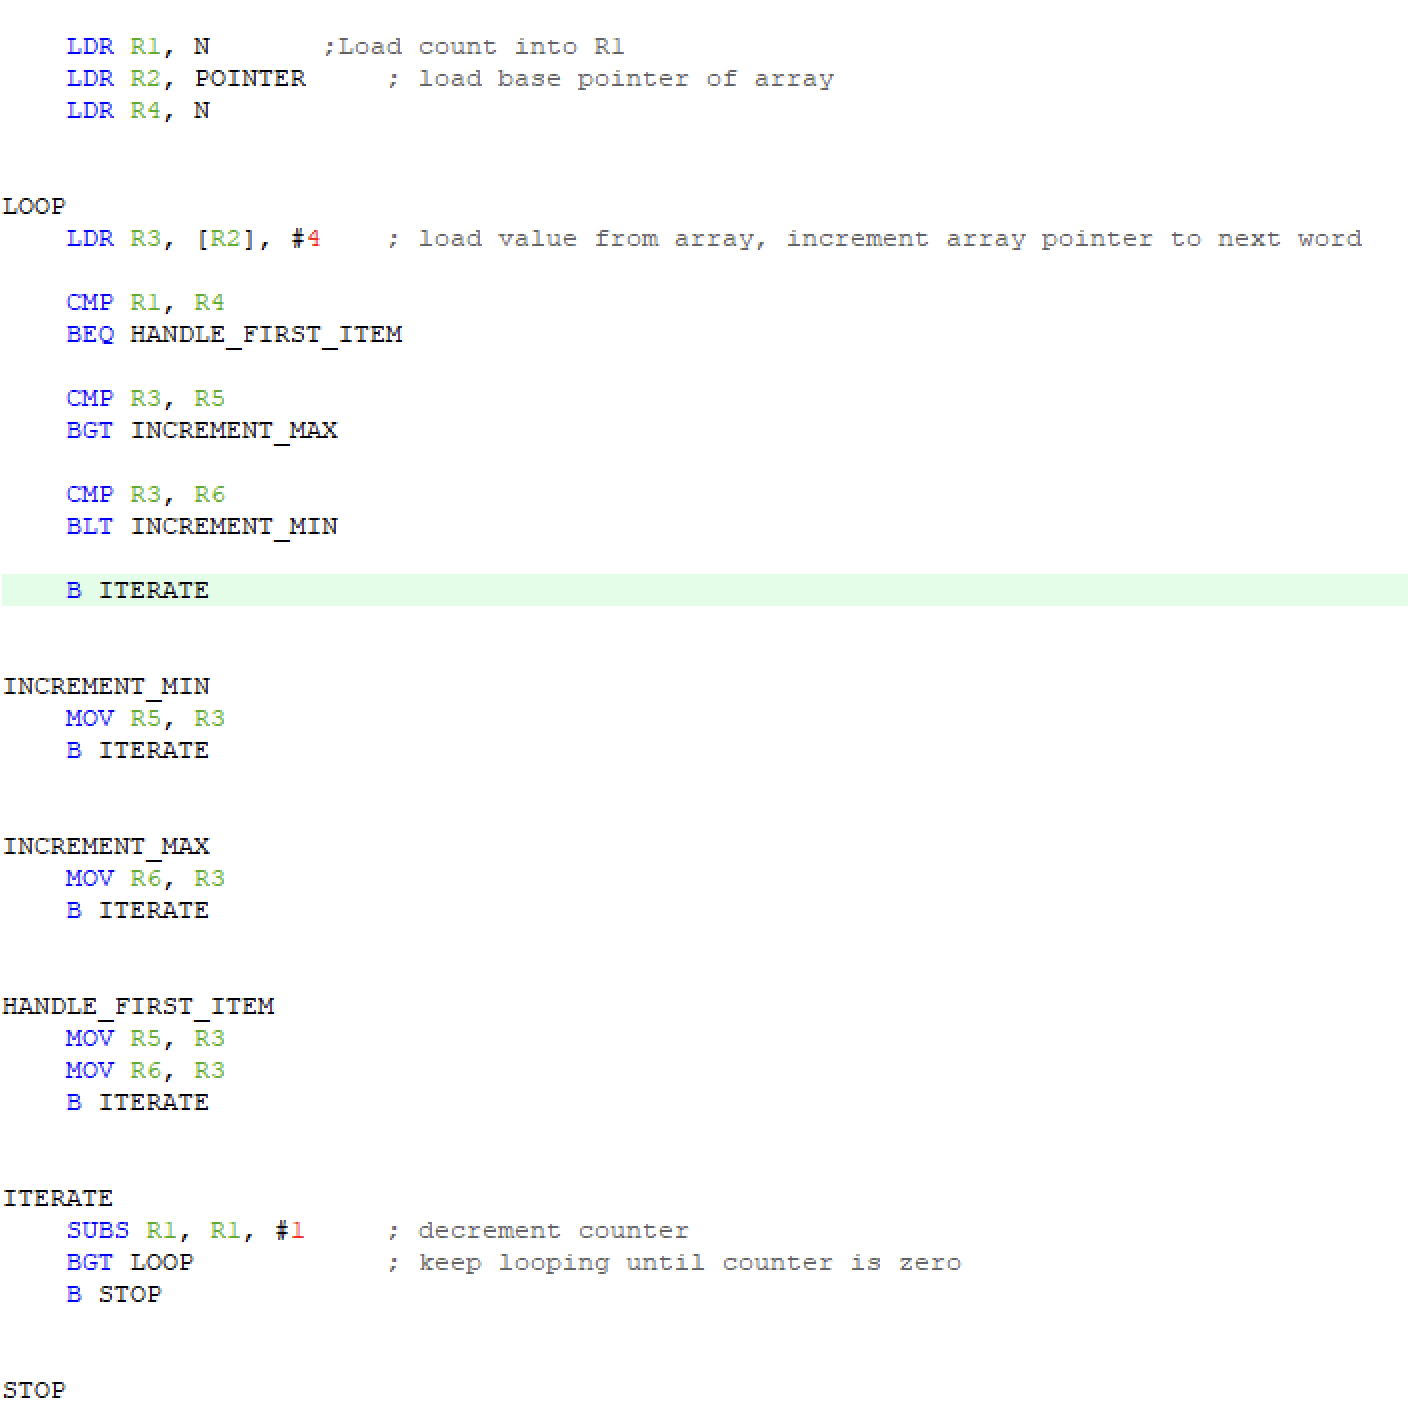
\includegraphics[width=\textwidth]{../Images/minMax_source_code.png}
\end{figure}

\begin{figure}
\caption{MinMax.s successful build}
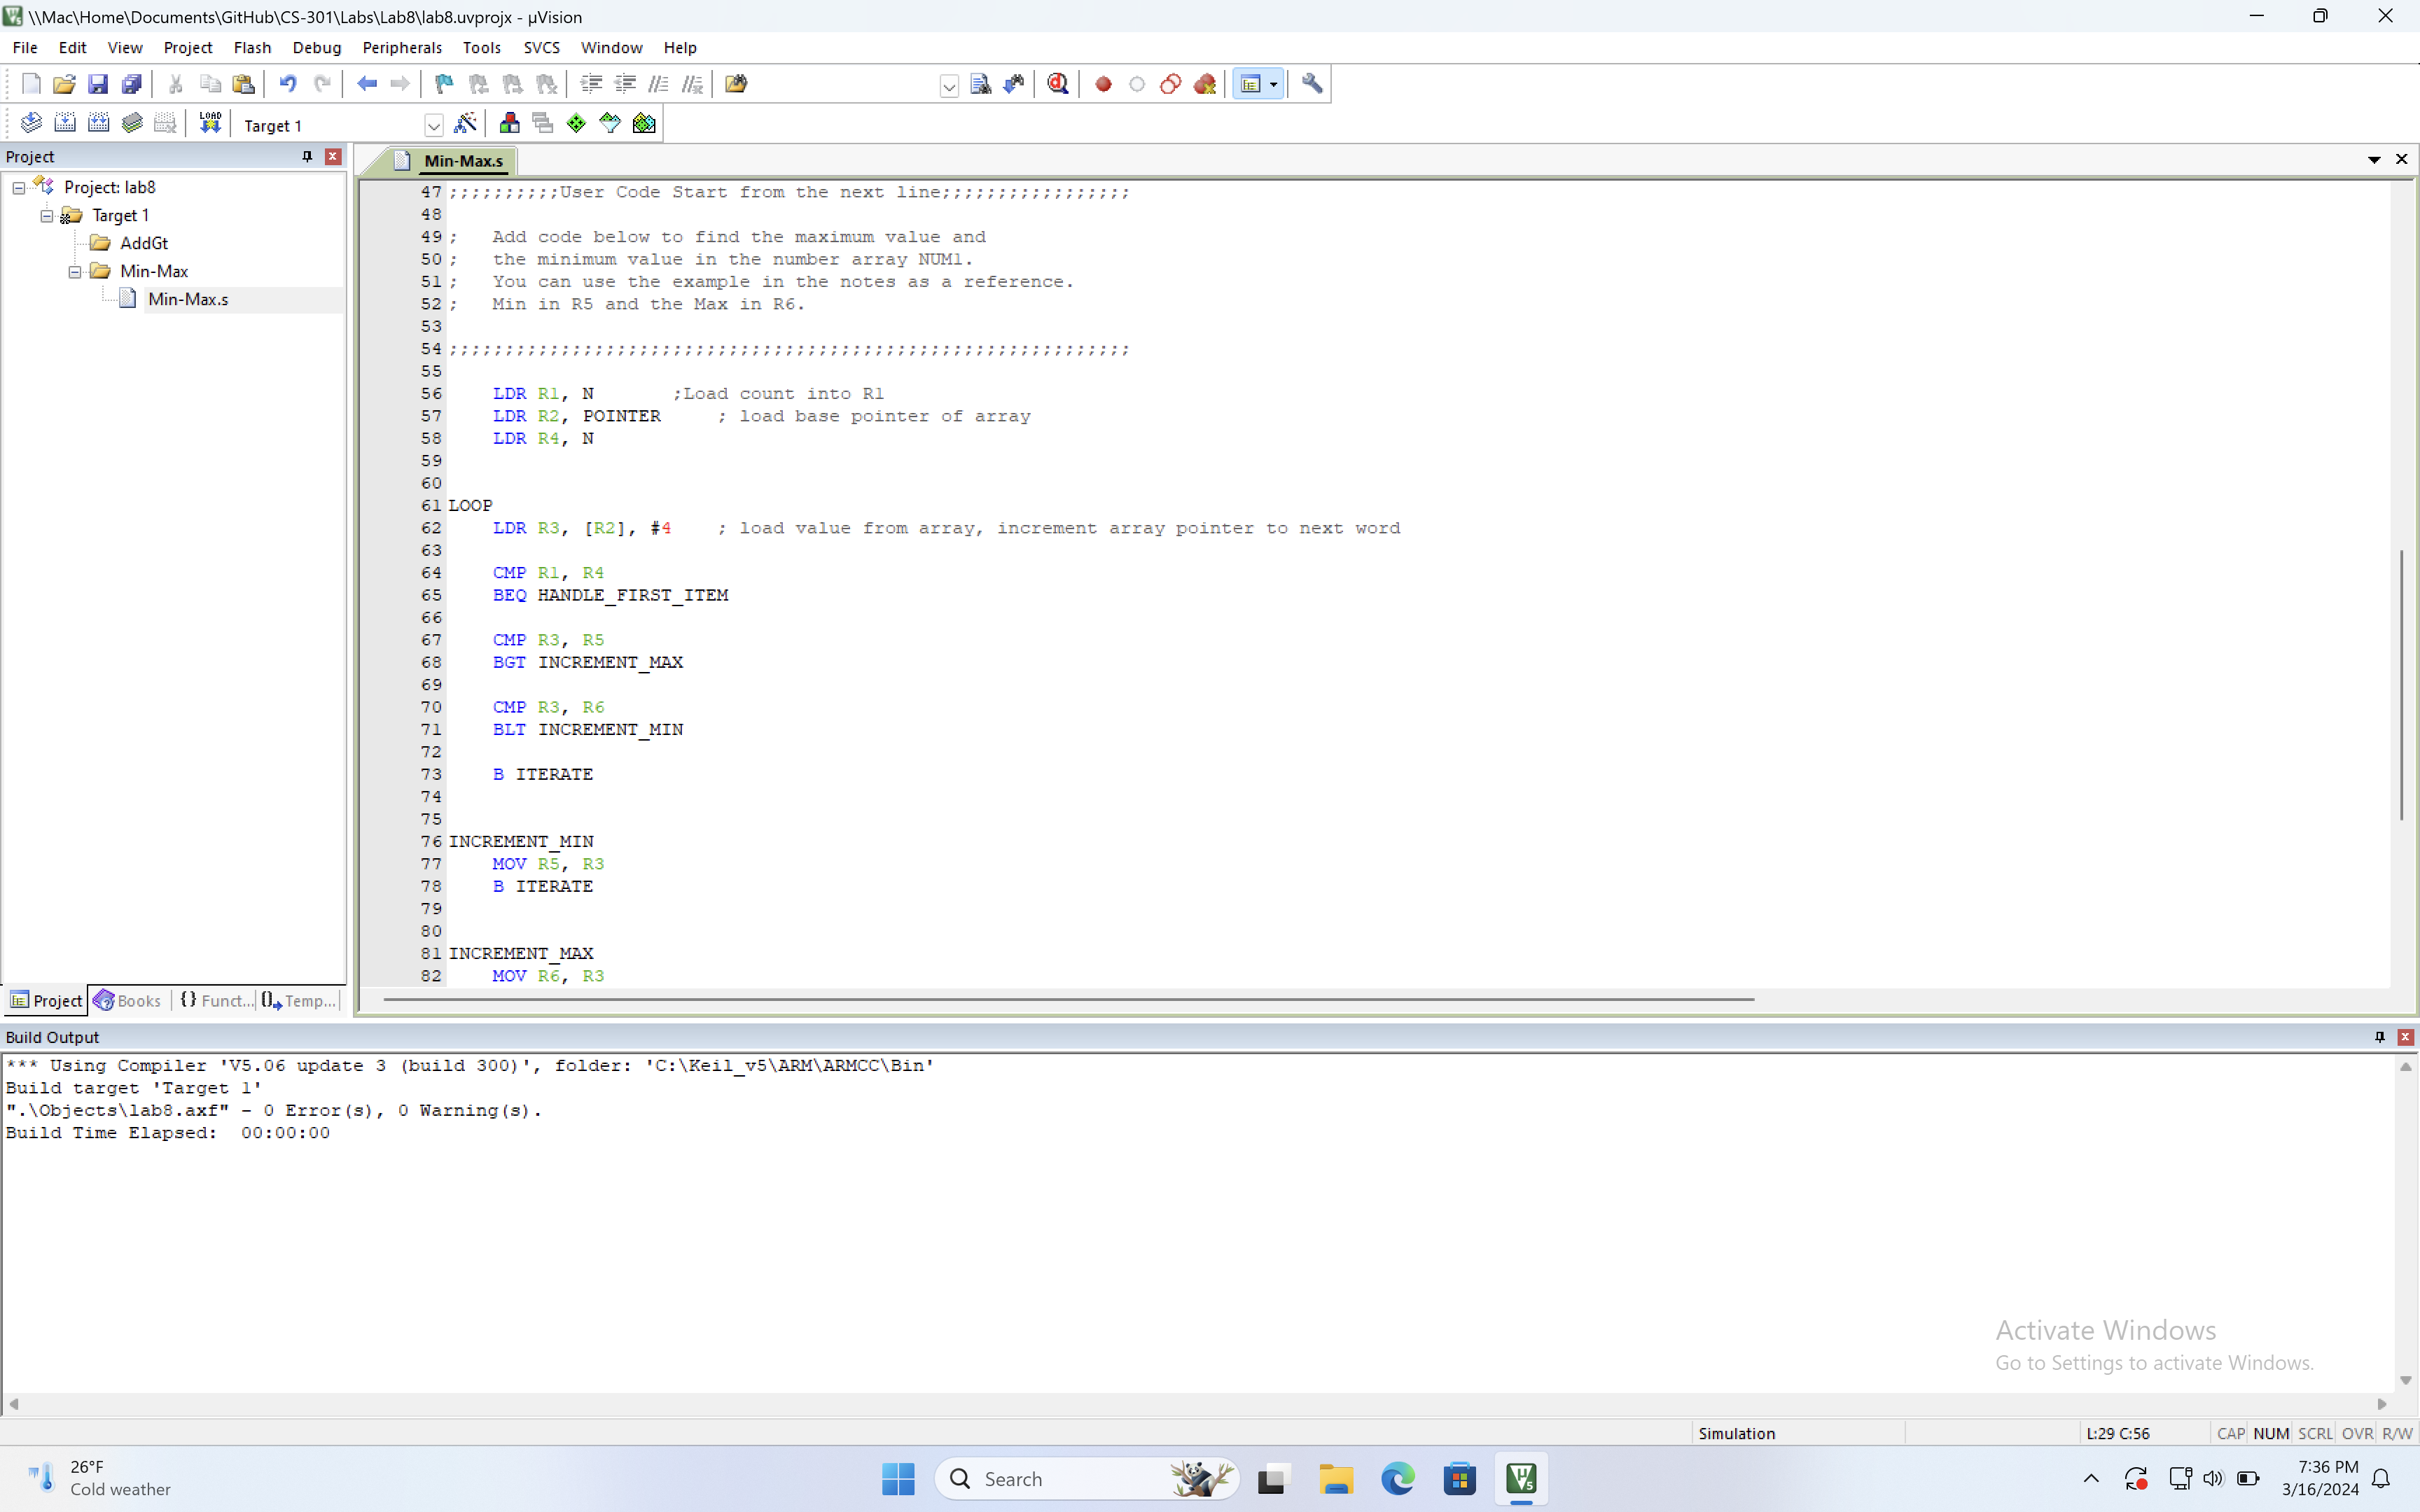
\includegraphics[width=\textwidth]{../Images/minMax_print_screen.png}
\end{figure}

\begin{figure}
\centering
\caption{MinMax.s Min in R5 and Max in R6}
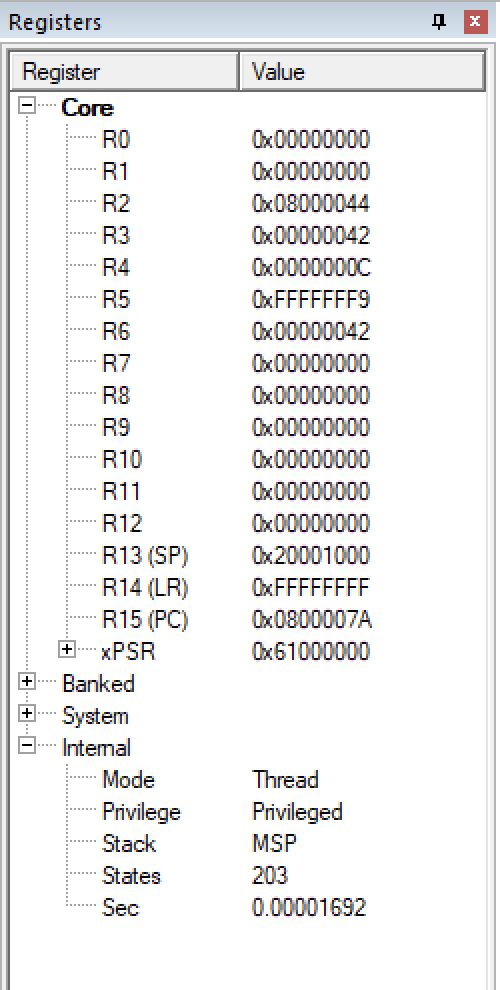
\includegraphics{../Images/minMax_register_vals.png}
\end{figure}

\end{document}